\documentclass[12pt]{article}  

\usepackage
[colorlinks=true, pdfstartview=FitV, linkcolor=blue, citecolor=blue, urlcolor=blue]
{hyperref}

\usepackage{amssymb}  
\usepackage{amsthm}
\usepackage{amsmath}
\usepackage{graphics} 
\usepackage{graphicx} 
%\usepackage[latin1]{inputenc}
\usepackage{tikz}
\usepackage{pgfplots}
\usepackage{wrapfig}
\usepackage{caption}
\usepgfplotslibrary{polar}
\usepackage{ skull }
\usetikzlibrary{decorations.fractals}


% GNUPLOT required
\usepackage{verbatim}

\linespread{1.3}

%\addtolength{\textwidth}{80pt}
\addtolength{\evensidemargin}{20pt}
\addtolength{\oddsidemargin}{20pt}

%%%%%%%%%%%%%%%%%%%%%%%%%%%%%%%%%%%%%%%%%%%%%%
%  Begin user defined commands

\newcommand{\map}[1]{\xrightarrow{#1}}

\newcommand{\N}{\mathbb N}
\newcommand{\Z}{\mathbb Z}
\newcommand{\Primes}{\mathbb P}
\newcommand{\Q}{\mathbb Q}
\newcommand{\R}{\mathbb R}
\newcommand{\C}{\mathbb C}
\newcommand{\bz}{\mathbb Z}
\newcommand{\bq}{\mathbb Q}
\newcommand{\br}{\mathbb R}
\newcommand{\bc}{\mathbb C}
\newcommand{\al}{\alpha}
\newcommand{\be}{\beta}
\newcommand{\ga}{\gamma}
\newcommand{\de}{\delta}
\newcommand{\ep}{\epsilon}
\DeclareMathOperator{\lub}{l.u.b.}
%  End user defined commands
%%%%%%%%%%%%%%%%%%%%%%%%%%%%%%%%%%%%%%%%%%%%%%


%%%%%%%%%%%%%%%%%%%%%%%%%%%%%%%%%%%%%%%%%%%%%%
% These establish different environments for stating Theorems, Lemmas, Remarks, etc.

\newtheorem{Thm}{Theorem}
\newtheorem{Prop}[Thm]{Proposition}
\newtheorem{Lem}[Thm]{Lemma}
\newtheorem{Cor}[Thm]{Corollary}

\theoremstyle{definition}
\newtheorem{Def}[Thm]{Definition}

\theoremstyle{remark}
\newtheorem{Rem}[Thm]{Remark}
\newtheorem{Ex}[Thm]{Example}

\theoremstyle{definition}
\newtheorem{Exercise}{Problem}

\newenvironment{Solution}{\noindent\textbf{Solution.}}{}

%\renewcommand{\labelenumi}{(\alph{enumi})}
\renewcommand\qedsymbol{QED}
% End environments 
%%%%%%%%%%%%%%%%%%%%%%%%%%%%%%%%%%%%%%%%%%%%%%%
%Some commands to save paper


\setlength{\parindent}{0in}
\setlength{\parskip}{8pt}

\DeclareMathOperator{\arcsec}{arcsec}
\DeclareMathOperator{\arccot}{arccot}
\DeclareMathOperator{\arccsc}{arccsc}
\DeclareMathOperator{\LH}{\ \underset{\text{LH}}{=}\ }
\newcommand{\Dep}{\Delta_+}
\newcommand{\Dem}{\Delta_-}
\newcommand{\bu}{\mathbf u}
\newcommand{\bv}{\mathbf v}
\newcommand{\bw}{\mathbf w}

\newcommand{\ora}{\overrightarrow}



\addtolength{\textwidth}{80pt}
\addtolength{\evensidemargin}{-40pt}
\addtolength{\oddsidemargin}{-40pt}
\addtolength{\topmargin}{-80pt}
\addtolength{\textheight}{1.8in}

\setlength{\parindent}{0in}
\setlength{\parskip}{8pt}

\DeclareMathOperator{\arcsinh}{arcsinh}

%%%%%%%%%%%%%%%%%%%%%%%%%%%%%%%%%%%%%%%%%%%%%%
% Now we're ready to start
%%%%%%%%%%%%%%%%%%%%%%%%%%%%%%%%%%%%%%%%%%%%%%

\begin{document}  

%\author{Your Name}
{\bf MATH 1103 Homework 4 Solutions}\\
{\bf Due Friday February 23, 2018}

Practice Problems (not to be turned in)

{\bf Practice 1.\ } Use an appropriate test to determine whether the following series converge or diverge.
\begin{enumerate}
\item[a)] $\sum\dfrac{10^k}{7+5^k}$,
\item[b)] $\sum\dfrac{5^{k+1}}{2+10^k}$,
\item[c)] $\sum\dfrac{\log k}{k}$,
\item[d)] $ \sum\dfrac{1}{n^n}$,
\item[e)] $ \sum\dfrac{1}{\sqrt{n^2+1}}$, 
\item[f)] $ \sum_{n=2}^\infty\dfrac{1}{\sqrt{n^2-1}}$, 
\item[g)] $ \sum k 3^{-k}$,
\item[h)] $ 1+\dfrac{1}{1\cdot 3}+\dfrac{1}{1\cdot 3\cdot 5}+\dfrac{1}{1\cdot 3\cdot 5\cdot 7}+\cdots $
\end{enumerate}

a)\ Diverges\quad 
b)\ Converges\quad 
c)\ Diverges\quad 
d)\ Converges\quad 
e)\ Diverges\quad 
f)\ Diverges\quad 
g)\ Converges\quad 
h)\ Converges\quad 

{\bf Practice 2.\ }  Give examples of the following:

a)\ a divergent series $\sum a_k$ with all $a_k>0$, such that $a_{k+1}/a_k< 1$. 

b)\ a  convergent series $\sum b_k$ with all $b_k>0$, such that $b_{k+1}/b_k< 1$. 

Then explain why a) and b)  do not contradict the Ratio Test. 

a) $\sum \dfrac{1}{k}$\quad  b) $\sum \dfrac{1}{k(k+1)}$

In both cases, the limit of the ratios is 1, so the Ratio Test does not apply. 

 \rule{\textwidth}{1pt}
The homework to be turned in may be found on the next page.


\newpage

{\bf Homework 4 problems to be turned in.}

{\bf 1.\ } In hw 3 you showed that $\sum\limits_{n=1}^\infty\dfrac{1}{n(n+1)}=1$. 
Use this sum and the Comparison Test to show that 
$\sum\limits_{n=1}^\infty\dfrac{1}{n^2}$ converges and that the sum is less than $2$. 
(Hint: The comparison test does not immediately apply. But rewrite the first sum to start at $n=2$.)

\begin{Solution} The first sum can be written as 
\[\sum\limits_{n=1}^\infty\dfrac{1}{n(n+1)}=
\sum\limits_{n=2}^\infty\dfrac{1}{n(n-1)}.
\]
The second sum is $1+\sum\limits_{n=2}^\infty\dfrac{1}{n^2}$. Since 
$\dfrac{1}{n^2}<\dfrac{1}{n(n-1)}$ for $n\geq 2$, the series 
$\sum\limits_{n=2}^\infty\dfrac{1}{n^2}$ converges. Since convergence is not affected by adding finitely many terms, the sum $\sum\limits_{n=1}^\infty\dfrac{1}{n^2}$ also converges

\end{Solution}

\rule{\textwidth}{1pt}\newline
{\bf Comment:\ } Imagine infinitely many equal masses placed at the points $0,1,2,\dots$. 
\begin{center}
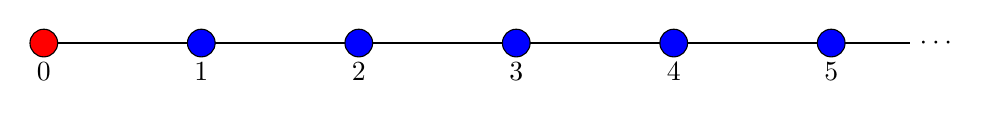
\begin{tikzpicture} [scale=2]
 \draw[black,-] (0,0) -- (5.5,0) node[right]{$\cdots$};
  \draw[fill=red] (0,0) circle (2.5pt);
  \draw[fill=blue] (1,0) circle (2.5pt);
   \draw[fill=blue] (2,0) circle (2.5pt);
    \draw[fill=blue] (3,0) circle (2.5pt);
     \draw[fill=blue] (4,0) circle (2.5pt);
     \draw[fill=blue] (5,0) circle (2.5pt);
 \node[label=below: $0$] at (0,0) {};   
  \node[label=below: $1$] at (1,0) {}; 
   \node[label=below: $2$] at (2,0) {}; 
    \node[label=below: $3$] at (3,0) {}; 
     \node[label=below: $4$] at (4,0) {}; 
         \node[label=below: $5$] at (5,0) {}; 
    \end{tikzpicture}
 \end{center}
With appropriate units of measurement, the series $\sum\limits_{n=1}^\infty\dfrac{1}{n^2}$  gives the gravitational force exerted on the mass at $0$ by all the other masses. Finding the sum was a famous problem, called the {\it Basel Problem} because  the Bernoulli family and Euler (all from Basel, Switzerland) worked on it. It was Euler who found the sum in 1734. Later, we'll see how he did it. 
\newline
\rule{\textwidth}{1pt}

{\bf 2.\ } Let $H_n$ be the $n^{th}$ harmonic number. We showed that 
$\log(n+1)<H_n<1+\log(n)$. 

a)\ Using a similar proof, show that 
$\dfrac{1}{n+1}<\log(n+1)-\log (n)<\dfrac{1}{n}$. 

b) Use the inequalities above to prove that the sequence $x_n=H_n-\log(n)$ converges and that the limit is between $0$ and $1$. 

(This limit, usually denoted by $\gamma$,  is called the {\bf Euler-Mascheroni constant}. We have $\gamma\approx .57721\dots$. No one knows if $\gamma$ is rational or irrational.) 

\begin{Solution} a) Look at the lower and upper rectangles for the graph of $1/x$ above the interval $[n,n+1]$. 

b)\ From the first inequalities, we have $0<H_n-\log(n+1)<H_n-\log n<1$, 
so $0<x_n<1$. From inequalities in a) we have 
\[x_n-x_{n+1}=(H_n-\log(n))-(H_{n+1}-\log(n+1))=\log(n+1)-\log n-\frac{1}{n+1}>0.\]
Therefore the sequence $(x_n)$ is decreasing and bounded between $0$ and $1$. 
By the Monotone Sequence Theorem, it converges, and the limit lies between $0$ and $1$. 


\end{Solution}

{\bf 3.\ } 
Around 1910, the Indian mathematician Srinivasa Ramanujan discovered that
\[
\frac{2\sqrt{2}}{9801}\sum_{n=0}^\infty\frac{(4n)!(1103+26390n)}{(n!)^4396^{4n}}=\frac{1}{\pi}.
\]
Prove the more modest assertion, that the series converges at all.

\begin{Solution} The constant $\dfrac{2\sqrt{2}}{9801}$ does not affect convergence, so we ignore it. For convenience, let $A=1103$, $B=26390$, $C=396$, so that 
\[a_n=\frac{(4n)!(A+Bn)}{(n!)^4C^{4n}}.\]
We apply the Ratio Test:
\[\begin{split}
\frac{a_{n+1}}{a_n}&=\frac{(4n+4)!(A+B+Bn)}{((n+1)!)^4C^{4n+4}}\cdot 
\frac{(n!)^4C^{4n}}{(4n)!(A+Bn)}\\
&=\frac{(4n+4)(4n+3)(4n+2)(4n+1)}{(n+1)^4}\cdot\frac{A+B+Bn}{C^4(A+Bn)}\\
&\to \left(\frac{4}{C}\right)^4.
\end{split}
\]
Since $C>4$, this limit is $<1$, so the series converges, by the ratio test. 
\end{Solution}

{\bf 4.\ } Using either the Comparison Test or the Ratio Test,  decide if the following series converge or diverge. 

a)\ $\sum\limits_{n=2}^\infty \dfrac{1}{\log n}$\qquad\qquad
b)\ $\sum\limits_{n=1}^\infty \dfrac{n!}{n^n}$\qquad\qquad
c)\ $1+\dfrac{1\cdot 2}{1\cdot 3}+\dfrac{1\cdot 2\cdot 3}{1\cdot 3\cdot 5}+
\dfrac{1\cdot 2\cdot 3\cdot 4}{1\cdot 3\cdot 5\cdot7}+\dots$

\begin{Solution} 

a)\ Diverges by comparison test with $\sum 1/n$. 

b)\ Converges by ratio test: 
\[\frac{a_{n+1}}{a_n}=\frac{(n+1)!}{(n+1)^{n+1}}\cdot\frac{ n^n}{n!}
=\frac{n^n}{(n+1)^n}=\left(\frac{n}{n+1}\right)^n=
\left(\frac{n+1}{n}\right)^{-n}=\left(1+\frac{1}{n}\right)^{-n}
\to \frac{1}{e}<1.
\]

c)\ Converges by the ratio test:
\[ 
\frac{a_{n+1}}{a_n}=\frac{n+1}{2n+1}\to \frac{1}{2}<1.\]
\end{Solution}
{\bf 5.\ }
a)\ Find all values of $x$ for which the series $\sum\limits_{k=1}^\infty\dfrac{x^n}{n}$ converges.

b)\ Find all values of $x$ for which the series $\sum\limits_{k=1}^\infty\dfrac{x^n}{n}$diverges.

\begin{Solution}
a)\ The series converges for $-1\leq x<1$. 
For if $-1<x<1$ then 
$\dfrac{|x|^{n+1}}{n+1}\cdot \dfrac{n}{|x|^n}=|x|\cdot \frac{n}{n+1}\to |x|<1$ 
So $\sum\dfrac{|x|^n}{n}$ converges, by the ratio test, and therefore $\sum\dfrac{x^n}{n}$ converges. 
If $x=-1$ then $\sum\dfrac{x^n}{n}=\sum\dfrac{(-1)^n}{n}$ converges by the alternating series test. 

b)\ The series diverges for $x<-1$ and $1\leq x$. For if $|x|>1$ then $x^n/n$ is unbounded, so cannot converge to zero. Hence $\sum\dfrac{x^n}{n}$ diverges. 
 If $x=1$ then $\sum\dfrac{x^n}{n}=\sum\dfrac{1}{n}$ is the Harmonic series, which also diverges.
 
 \end{Solution}




\newpage
{\bf 6.\ } The {\bf Koch snowflake} is a fractal (when you zoom in, it looks the same) constructed from an expanding sequence of polygons  as follows. 

Step 0. Start with an equilateral triangle $K_0$. 

Step 1. Replace the middle third of each side of $K_0$ with equilateral triangles, making a 12-sided polygon $K_1$.

Step 2. Replace the middle third of each side of $K_1$ with equilateral triangles, making a 48-sided polygon $K_2$. 

Step $n$. Replace the middle third of each side of $K_{n-1}$ with equilateral triangles to obtain $K_n$. 

The first few polygons $K_0,\dots, K_4$ are shown below. The Koch snowflake is the union of all the polygons $K_n$. The area of $K$ is the limit of the areas of the polygons $K_n$:
\[\text{area}(K)=\lim_{n\to\infty}\text{area}(K_n).\]

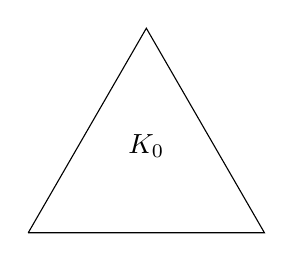
\begin{tikzpicture}[decoration=Koch snowflake]
   \draw 
        (0,0) -- ++(60:3)  -- ++(300:3) -- ++(180:3);
   \node[label=below: $K_0$] at (1.5,1.5) {};     
\end{tikzpicture}\quad
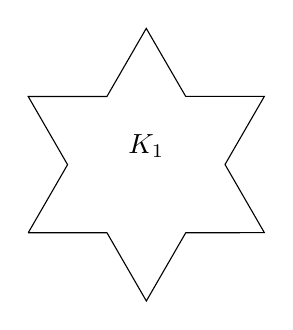
\begin{tikzpicture}[decoration=Koch snowflake]
   \draw decorate{  
        (0,0) -- ++(60:3)  -- ++(300:3) -- ++(180:3)};
        \node[label=below: $K_1$] at (1.5,1.5) {};
\end{tikzpicture}\quad
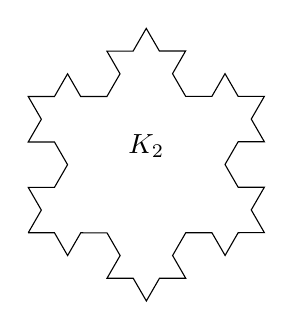
\begin{tikzpicture}[decoration=Koch snowflake]
   \draw decorate{ decorate{ 
        (0,0) -- ++(60:3)  -- ++(300:3) -- ++(180:3)}};
        \node[label=below: $K_2$] at (1.5,1.5) {};
\end{tikzpicture}\quad
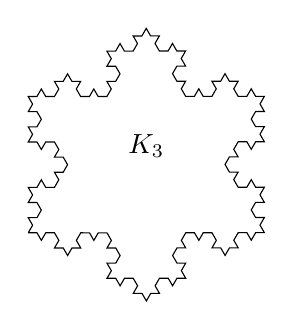
\begin{tikzpicture}[decoration=Koch snowflake]
   \draw decorate{ decorate{ decorate{ 
        (0,0) -- ++(60:3)  -- ++(300:3) -- ++(180:3)}}};
        \node[label=below: $K_3$] at (1.5,1.5) {};
\end{tikzpicture}\quad
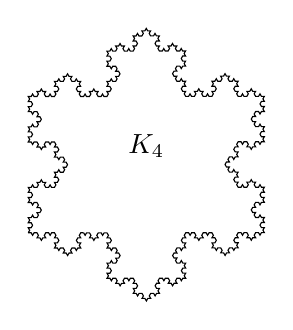
\begin{tikzpicture}[decoration=Koch snowflake]
   \draw decorate{ decorate{ decorate{ decorate{
        (0,0) -- ++(60:3)  -- ++(300:3) -- ++(180:3)}}}};
        \node[label=below: $K_4$] at (1.5,1.5) {};
\end{tikzpicture}\quad
%\begin{tikzpicture}[decoration=Koch snowflake]
   %\draw decorate{ decorate{ decorate{ decorate{ decorate{
       % (0,0) -- ++(60:3)  -- ++(300:3) -- ++(180:3)}}}}};
%\end{tikzpicture}\quad
Let $T_n$ be the number of triangles added at the $n^{th}$ step. (So $T_0=1, T_1=3, T_2=12,\dots$.). And let $A_n$ be the  area of each triangle added at step $n$. (So $A_0=\text{area}(K_0), A_1=\frac{1}{9}A_0,\dots$). 

a) Find formulas for $T_n$ and $A_n$, in terms of $n$. 

b)\ Compute $\text{area}(K_n)$. 

c)\ Use the geometric series to find $\text{area}(K)$. 


\begin{Solution}

a)\ Each edge gives four new edges at the next step, so $T_0=1$ and 
$T_n=3\cdot 4^{n-1}$ for $n\geq 1$. 
Each new triangle has side one-third of the previous triangles, hence has $1/9$ of the area of the previous triangles. So $A_n=(1/9)^{n}A_0$. 

b)\ 
\[\begin{split}
\text{area}(K_n)&=\sum_{k=0}^n T_k A_k\\
&=A_0+\sum_{k=1}^n 3\cdot 4^{k-1}\cdot \frac{1}{9^k}A_0\\
&=A_0\left [1+\frac{1}{3}\sum_{k=0}^{n-1}\left(\frac{4}{9}\right)^k\right]\\
&=A_0\left [1+\frac{1}{3}\cdot \frac{1-(4/9)^{n}}{1-(4/9)}\right].
\end{split}
\]

c)\ Taking the limit as $n\to\infty$, we get
\[\text{area}(K)=\lim_{n\to\infty}
\text{area}(K_n)=A_0\left [1+\frac{1}{3}\frac{1}{1-(4/9)}\right]
=\frac{8}{5}\cdot A_0.
\]

\end{Solution}
\end{document}









\end{document}

 
 
